\documentclass[aspectratio=169]{beamer}
\usepackage[spanish]{babel} % Define el idioma del documento
\usepackage{listings}
\usepackage{tikz}
\usetikzlibrary{positioning}
\usepackage{hyperref} % Utilizado para crear hipervínculos en el documento
\hypersetup{
	colorlinks=true,
	linkcolor=blue,
	filecolor=magenta,
	urlcolor=cyan,
}

\lstset{%
  frame            = tb,    % draw frame at top and bottom of code block
  tabsize          = 1,     % tab space width
  framesep         = 3pt,   % expand outward
  framerule        = 0.4pt, % expand outward 
  commentstyle     = \color{Green},      % comment color
  keywordstyle     = \color{blue},       % keyword color
  stringstyle      = \color{DarkRed},    % string color
  backgroundcolor  = \color{lightgray}, % backgroundcolor color
  showstringspaces = false,              % do not mark spaces in strings
}

\usetheme{unad}

\title{Preparación de Documentos Técnicos Usando \LaTeX}
\author{Gerardo Becerra, Ph.D.}
\institute{UNAD}
\date{Febrero 26 de 2022}
\institute{Escuela de Ciencias Básicas, Tecnología e Ingeniería}
\city{Bogotá D.C.}

\usebackgroundtemplate%
{%
    
\includegraphics[width=\paperwidth,height=\paperheight]{img/content_background.jpg}%
}

\AtBeginSection[]
{
	\begin{frame}<beamer>
		\frametitle{Agenda de la Presentación}
		\tableofcontents[currentsection]
	\end{frame}
}


\begin{document}

% Diapositiva de título
{\usebackgroundtemplate{
	
\includegraphics[width=\paperwidth]{img/cover_background.jpg}}%
	\frame{\titlepage}
}

% Aquí inician los contenidos de la presentación
\section{Introducción al sistema \LaTeX}
\begin{frame}[t]\frametitle{¿Qué es \LaTeX?}
	\begin{itemize}
		\item Es un lenguaje creado por \href{https://en.wikipedia.org/wiki/Donald_Knuth}{Donald Knuth} y luego extendido por \href{https://en.wikipedia.org/wiki/Leslie_Lamport}{Leslie Lamport} para crear documentos atractivos y consistentes.
		\item Es un lenguaje tipográfico y de marcado (markup):
		\begin{itemize}
			\item Tipográfico: Reglas que definen la organización y presentación de los contenidos en un documento.
			\item Marcado: Reglas que definen los contenidos de un documento.
		\end{itemize}
		\item Estos dos aspectos se manejan por separado (Una persona crea la plantilla y otra se encarga de producir los contenidos del documento).
	\end{itemize}
\end{frame}

\begin{frame}[t]\frametitle{¿Por qué usar \LaTeX?}
	\begin{itemize}
		\item Dos enfoques diferentes:
		\begin{itemize}
			\item Sistemas \emph{What You See is What You Get} (WYSIWYG): Microsoft Word, Google Docs, LibreOffice, etc. $\longrightarrow$ A medida que se va editando el documento se  va observando la apariencia que éste toma. 
			\item \LaTeX\ $\longrightarrow$ Se utilizan comandos para describir los contenidos en un archivo de texto, y luego un programa se encarga de producir el documento.
		\end{itemize}
	\end{itemize}	
\end{frame}

\begin{frame}[t]\frametitle{¿Por qué usar \LaTeX?}
	\begin{itemize}
		\item Ventajas:
		\begin{itemize}
			\item El autor se puede concentrar únicamente en la estructura y contenidos del documento. \LaTeX\ se encarga de aplicar las reglas tipográficas para producir un documento consistente.
			\item En \LaTeX\ es fácil reproducir la estructura de un documento.
			\item Manejo automático de índices, pies de página, citaciones y referencias.
			\item Las fórmulas matemáticas se pueden preparar fácilmente.
			\item El documento de origen es texto plano
			\begin{itemize}
			 	\item Lectura en cualquier sistema
			 	\item Generación automática de contenidos
			 	\item Control de versiones
			 \end{itemize}
			\item La preparación de artículos para revistas y conferencias internacionales se realiza usando plantillas de \LaTeX.
			\item ¡Es gratuito!
		\end{itemize}
	\end{itemize}
\end{frame}

\begin{frame}[t]\frametitle{¿Cómo obtener \LaTeX?}
	\begin{itemize}
		\item Para empezar, ¡no se requiere instalar nada! $\longrightarrow$ Editor en línea: \href{https://www.overleaf.com}{Overleaf}.
		\item Para trabajar fuera de línea, se descarga y se instala una distribución de \LaTeX:
		\begin{itemize}
			\item \href{http://www.tug.org/texlive/}{TeX Live}: Distribución multiplataforma.
			\item \href{http://www.miktex.org/}{MiKTeX}: Distribución multiplataforma.
			\item \href{http://www.tug.org/mactex/}{MacTeX}: Distribución para Mac OS, basada en TeX Live.
		\end{itemize}
		\item Para preparar los documentos se requiere un \href{https://en.wikipedia.org/wiki/Comparison_of_TeX_editors}{editor de texto}.
		\item Para usar funcionalidades específicas, se pueden instalar \href{https://www.ctan.org/}{paquetes adicionales}.
	\end{itemize}
\end{frame}

\section{Fundamentos de \LaTeX}
\begin{frame}[fragile]\frametitle{La Sintaxis de \LaTeX}
\begin{columns}
	\begin{column}{0.5\textwidth}
		Para crear un documento se puede utilizar cualquier editor de texto. A continuación se encuentra un ejemplo mínimo:
		\begin{lstlisting}[backgroundcolor=\color{lightgray}]
\documentclass{article}
% Preambulo
\begin{document}
  Contenidos del documento...
\end{document}	
		\end{lstlisting}
	\end{column}
	\begin{column}{0.5\textwidth}
		El documento obtenido será el siguiente:
		\begin{figure}
			\centering
			
\includegraphics[width=\textwidth]{img/ejemplo_minimo.png}
		\end{figure}
	\end{column}
\end{columns}
\end{frame}

\begin{frame}[fragile]\frametitle{Espacios en Blanco}
	\begin{columns}
		\begin{column}{0.5\textwidth}
			\begin{itemize}
				\item El compilador de \LaTeX\ normaliza los espacios en blanco. Varios caracteres consecutivos de [espacio] y [tabulador] son tratados como uno sólo.
				\item Un salto de línea sencillo [Enter] también es tratado como un espacio en blanco.
				\item Dos saltos de línea definen un nuevo párrafo.
			\end{itemize}
		\end{column}
		\begin{column}{0.5\textwidth}
			\begin{lstlisting}[backgroundcolor=\color{lightgray}]
No importa si se introducen
uno o mas            espacios
despues de una	palabra.

Una linea vacia siempre
inicia un nuevo parrafo.
			\end{lstlisting}
			\begin{figure}
				\centering
				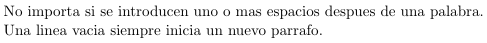
\includegraphics[width=\textwidth]{img/espacio_blanco.png}
			\end{figure}
		\end{column}
	\end{columns}	
\end{frame}

\begin{frame}[fragile]\frametitle{Caracteres Reservados}
	\begin{itemize}
		\item Los siguientes símbolos son de uso reservado y si se introducen directamente en el texto pueden generar errores: \#\ \$\ \%\ \^\ \&\ \_\ \{\ \}\ \~\ \textbackslash{}.
		\item Para utilizarlos dentro del texto se adiciona el caracter \textbackslash{} de la siguiente manera:
		\begin{lstlisting}[backgroundcolor=\color{lightgray}]
\# \$ \% \^ \& \_ \{ \} \~ \textbackslash{}
		\end{lstlisting}
	\end{itemize}
\end{frame}

\begin{frame}[fragile]\frametitle{Entornos de \LaTeX (Environments)}
	\begin{itemize}
		\item Son estructuras que definen las características locales de los contenidos en el documento.
		\item Su sintaxis se define de la siguiente manera:
		\begin{lstlisting}[backgroundcolor=\color{lightgray}]
\begin{nombreentorno}
  Texto o contenidos que van a ser influenciados
\end{nombreentorno}
		\end{lstlisting}
	\end{itemize}
\end{frame}

\begin{frame}[fragile]\frametitle{Comandos de \LaTeX}
	\begin{itemize}
		\item Los comandos inician con el caracter backslash \textbackslash{} y continúan con el nombre.
		\item Algunos comandos requieren un argumento que se debe dar dentro de llaves \{\ \}.
		\item La sintáxis general es:
		\begin{lstlisting}[backgroundcolor=\color{lightgray}]
\nombrecomando[opcion1,opcion2,...]{argum1}{argum2}...
		\end{lstlisting}
	\end{itemize}
\end{frame}

\begin{frame}[fragile]\frametitle{Comentarios}
	\begin{itemize}
		\item El caracter \% se utiliza para representar comentarios dentro del archivo de texto.
		\item \LaTeX\ ignora el contenido que se encuentra después del caracter \% y no lo incluye en el documento preparado.
		\item \LaTeX\ también ignora el salto de línea y todo el espacio en blanco al inicio de la siguiente línea.
	\end{itemize}
	\begin{columns}
		\begin{column}{0.5\textwidth}
			\begin{lstlisting}[backgroundcolor=\color{lightgray}]
% Este texto no es mostrado
% Este tampoco
Este texto si es visible

Otra linea de % comentario
       contenido
			\end{lstlisting}
		\end{column}
		\begin{column}{0.5\textwidth}
			\begin{figure}
				\centering
				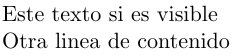
\includegraphics[width=4cm]{img/comentarios.png}
			\end{figure}
		\end{column}
	\end{columns}
\end{frame}

\begin{frame}[t]\frametitle{Generar el Documento}
	\begin{itemize}
		\item Los archivos de texto fuente de \LaTeX\ se guardan con la extensión \texttt{tex} (p.ej. \texttt{hola.tex}
		\item Para compilar el archivo de texto fuente se utiliza el comando \texttt{latex} junto con el nombre del archivo (p.ej. \texttt{latex hola}. Éste comando producirá un archivo con extensión \texttt{dvi} (p.ej. \texttt{hola.dvi}).
		\item Luego, para generar el archivo final en formato \texttt{pdf} se utiliza el comando \texttt{pdflatex} (p.ej. \texttt{pdflatex hola}).
		\item Si se utiliza un editor de texto estos comandos se ejecutan de manera automática.
		\item También existen sistemas para realizar la compilación en un sólo paso. Por ejemplo \texttt{latexmk -pdf hola.tex}.
		\item El proceso de compilación produce algunos archivos auxiliares (\texttt{aux}, \texttt{log}, \texttt{fls}, \texttt{nav}, etc).
	\end{itemize}
\end{frame}


\section{Estructura del Documento}
\begin{frame}[t]\frametitle{Estructura General del Documento}
	\begin{itemize}
		\item Para comunicar mejor nuestras ideas, nuestros textos deben tener una estructura lógica.
		\item \LaTeX\ requiere que el autor indique la estructura lógica del contenido para preparar el documento de acuerdo a las reglas de \emph{typesetting}.
		\item \LaTeX\ permite utilizar estructuras jerárquicas tales como capítulos, secciones, subsecciones y parágrafos.
	\end{itemize}
\end{frame}

\begin{frame}[fragile]\frametitle{Estructura General del Documento}
    
\begin{lstlisting}[numbers = none, escapechar = !,
    basicstyle = \ttfamily\bfseries, linewidth = .6\linewidth] 
 \documentclass[options]{class} !\tikz[remember picture] \node [] (a) {};!

 		\includepackage{package1} !\tikz[remember picture] \node [] (b){};!           
 		\includepackage{package2}
    
 		\begin{document} !\tikz[remember picture] \node [] (c){};! 

 				Contenidos !\tikz[remember picture] \node [] (d){};!  

		\end{document} !\tikz[remember picture] \node [] (e){};!
 % }
\end{lstlisting}
\begin{tikzpicture}[remember picture, overlay,
    every edge/.append style = { ->, thick, >=stealth,
                                  gray, dashed, line width = 1pt },
    every node/.append style = { align = center, minimum height = 10pt,
                                 font = \bfseries, fill= green!20},
                  text width = 5cm ]
  \node [right = 1.1cm of a]  (A) {Clase del documento};
  \node [right = 1.8cm of b]  (B) {Preámbulo};
  \node [right = 4.0cm of c]  (C) {Inicio entorno documento};
  \node [right = 5.0cm of d]  (D) {Contenidos del documento};  
  \node [right = 4.7cm of e]  (E) {Fin entorno documento};  
  \draw (A.west) edge (a.east);
  \draw (B.west) edge (b.east) ;
  \draw (C.west) edge (c.east) ;  
  \draw (D.west) edge (d.east) ;
  \draw (E.west) edge (e.east) ;
\end{tikzpicture}
\end{frame}

\begin{frame}[t]\frametitle{Clases de Documentos}
	\centering
	\begin{tabular}{ll}
		\hline
		\textbf{Clase} & \textbf{Descripción}\\
		\hline
		\texttt{article} & Artículos de revista, reportes, documentación, etc\\
		\texttt{IEEEtran} & Artículos con formato IEEE Transactions\\
		\texttt{report} & Reportes largos con varios capítulos, libros cortos, tesis\\
		\texttt{book} & Libros\\
		\texttt{letter} & Cartas\\
		\texttt{beamer} & Presentaciones\\
		\hline
	\end{tabular}
\end{frame}

\begin{frame}[t]\frametitle{Ejercicio 1}
	\begin{itemize}
	 	\item Crea un documento usando la clase \texttt{article} donde se incluya título, autor y fecha. Configura el papel en tamaño carta. Utiliza el paquete \texttt{lipsum} para generar textos genéricos.
	 	\item Modifica el documento anterior para configurar el papel en tamaño A4 y organizar el texto en doble columna. Cambia el tamaño base del tipo de letra a 12 puntos.
	\end{itemize} 
\end{frame}

\begin{frame}[fragile]\frametitle{Resumen del Documento}
	En muchas situaciones, se requiere introducir un resumen (abstract) al inicio del documento. Para hacerlo se usa el entorno \texttt{abstract}:
	\begin{lstlisting}[backgroundcolor=\color{lightgray}]
\begin{abstract}
	Escribe aqui tu resumen...
\end{abstract}
	\end{lstlisting}
\end{frame}

\begin{frame}[t]\frametitle{Ejercicio 2}
	\begin{itemize}
	 	\item Modifica el documento anterior para agregar un resumen. Usa el paquete \texttt{lipsum} para generar los textos.
	\end{itemize} 
\end{frame}

\begin{frame}[t]\frametitle{Secciones del Documento}
	La estructura lógica de un documento puede dividirse en una jerarquía de partes, capítulos, secciones, parágrafos, etc. En la siguiente tabla se muestran los diferentes niveles y los comandos a utilizar:\\
	\begin{table}
		\centering
		\begin{tabular}{lc}
			\hline
			\textbf{Comando} & \textbf{Nivel}\\
			\hline
			\texttt{\textbackslash{}part\{parte\}} & -1\\
			\texttt{\textbackslash{}chapter\{capítulo\}} & 0\\
			\texttt{\textbackslash{}section\{sección\}} & 1\\
			\texttt{\textbackslash{}subsection\{subsección\}} & 2\\
			\texttt{\textbackslash{}subsubsection\{subsubsección\}} & 3\\
			\texttt{\textbackslash{}paragraph\{parágrafo\}} & 4\\
			\texttt{\textbackslash{}subparagraph\{subparágrafo\}} & 5\\
			\hline
		\end{tabular}
	\end{table}
\end{frame}


\begin{frame}[t]\frametitle{Ejercicio 3}
	\begin{itemize}
	 	\item Crea un artículo que incluya los siguientes elementos: título, autor, fecha, abstract, tabla de contenido y contenido. Organiza el contenido en las secciones introducción, metodología, resultados y conclusiones. Utiliza el paquete \texttt{lipsum} para generar los textos.
	 	\item Crea un libro que tenga 3 capítulos, cada uno con 2 secciones. El libro debe tener una portada con el título, autor y fecha. También debe incluir la tabla de contenido.
	\end{itemize} 
\end{frame}


% Diapositiva final
{\usebackgroundtemplate{
	
\includegraphics[width=\paperwidth]{img/end_background.jpg}}%
	\begin{frame}
		\vskip3.2cm
		\centering
		\LARGE\textcolor{myblue}{\textbf{¡GRACIAS!}}
	\end{frame}
	
}

\end{document}